\chapter{Preliminari}

\section{Diagrammi e tabelle}

\begin{defn}[Diagramma di Young]
Un diagramma di Young $\lambda=(n_1,n_2,\dots,n_k)$ \`e una
rappresentazione di una partizione di un intero positivo $n =
\sum_{i=0}^{k}{n_i}$ come somma di interi positivi $n_k \geq \ldots \geq
n_2 \geq n_1 \geq 0$. Graficamente possiamo immaginare un diagramma di
Young come $k$ righe di celle quadrate, allineate a sinistra, di
lunghezza $n_k,\ldots,n_2,n_1$ dall'alto verso il basso in quest'ordine.
\end{defn}

\begin{defn}[Diagramma coniugato]
Dato un diagramma di Young $\lambda=(n_1,n_2,\dots,n_k)$, definiamo il
suo coniugato $\tilde{\lambda}$ come il diagramma che ha le colonne di
lunghezza $n_k,\ldots,n_2,n_1$ da sinistra verso destra in quest'ordine.  
\end{defn}

\begin{figure}[h]
\centering

\begin{subfigure}[b]{0.4\textwidth}
\centering
\includegraphics[height=0.35\textwidth]{YoungDiagram}
\caption{$\lambda=(1,1,2,3,4)$}
%% \label{fig:awesome_image}
\end{subfigure}%
\begin{subfigure}[b]{0.4\textwidth}
\centering
\raisebox{0.2\height}{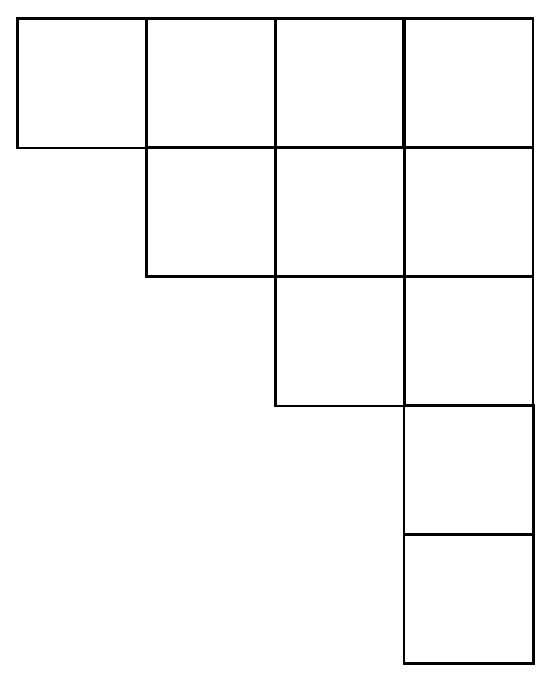
\includegraphics[height=0.35\textwidth,angle=90]{YoungDiagramFlip}}
\caption{$\tilde{\lambda}=(1,2,3,4)$}
\end{subfigure}
\caption{Un diagramma di Young ed il suo coniugato.}
\end{figure}

Possiamo calcolare il diagramma coniugato con la funzione
\emph{ydiagram\_transpose\_rows}:

\begin{alltt}
\emph{remove\_diagram\_column} (r, l) := 
if emptyp (r) then return (l)
else block (
  l : append ([length (r)], l),
  r : r-1,
  r : delete (0, r),
  return (\emph{remove\_diagram\_column} (r, l)));

\emph{ydiagram\_transpose\_rows} (d) := \emph{remove\_diagram\_column} (d, []);
\end{alltt}

La funzione \emph{remove\_diagram\_column} toglie la colonna pi\`u a
sinistra del diagramma e la inserisce come ultima riga del diagramma coniugato.

\begin{notaz}
Scriveremo $\lambda \vdash n$ intendendo che $\lambda$ \`e una
partizione di $n$.
\end{notaz}

Diremo che un diagramma $\mu=(n_1,n_2,\dots,n_k)$ \emph{\`e pi\`u
piccolo} di un diagramma $\lambda=(m_1,m_2,\dots,m_h)$, e scriviamo
$\mu \subset \lambda$, se

\begin{enumerate}[(i)]
\item $k \leq h$;
\item $n_i \leq m_i$ per ogni $1 \leq i \leq k$.
\end{enumerate}

\begin{defn}[Skew diagram]
Uno skew diagram \`e il diagramma che si ottiene togliendo un
diagramma di Young $\mu$ da un diagramma $\lambda$ che lo contiene
\end{defn}

\begin{defn}[Tabella di Young]\label{ytab}
Diremo Young tableau un riempimento di un diagramma di Young con
numeri interi positivi che risulti:
\begin{enumerate}[(i)]
\item non decrescente lungo le righe;
\item strettamente crescente lungo le colonne.
\end{enumerate}
Un Young tableau si dice \emph{standard} se il riempimento di
$\lambda \vdash n$ \`e composto dai primi $n$ interi positivi (non
ripetuti).
\end{defn}

\begin{oss}
Un Young tableau standard \`e strettamente crescente \emph{anche}
lungo le righe.
\end{oss}

\begin{oss}
Ogni tabella $T$ \`e riempimento di un unico diagramma $\lambda$. Il
diagramma di cui $T$ \`e riempimento \`e detto \emph{forma di $T$}
\end{oss}

\begin{defn}[Skew tableau]
Diremo skew tableau un riempimento di uno skew diagram che rispetti i
requisiti della definizione \ref{ytab}. 
\end{defn}

\section{Row bumping}
Il row bumping \`e la procedura con la quale dati un tableau $T$ e un
intero positivo $x$ si costruisce un tableau, che indicheremo con $T
\gets x$, la cui forma ha un box in pi\`u della forma di $T$ con
entrata $x$.\\
Se $x_1 = x$ \`e non minore di ciascun elemento della prima riga
dall'alto di $T$, aggiungiamo alla fine di tale riga l'entrata x.
Altrimenti se $x_2$ \`e il primo elemento da sinistra della prima riga
di $T$ strettamente maggiore di $x_1$, inseriamo $x_1$ al posto di
$x_2$ e procediamo al suo inserimento nella seconda riga di $T$.
Ripetiamo quindi per le successive righe, fino a quando non siamo in
grado di effettuare un inserimento al termine di una riga oppure fino
a quando aggiungeremo una riga in basso contenente l'elemento $x_h$
sostituito nell'ultima riga al passo precedente con l'elemento
$x_{h-1}$.

\begin{figure}[h]
\centering
\includegraphics[width=0.8\textwidth]{row_bump}
\caption{Row bumping}
\end{figure}

\begin{alltt}
/* rb should be [r, x] where x is the element that is being bumped */
/* in the row r */
/* i should be length (r) */
/* rec\_bump\_row returns [bumped\_row, next\_x] or [append (r,[x]), 0]  */
\emph{rec\_bump\_row} (r, x, i) :=
if (x >= last (r)) then [append (r, [x]), 0] /* r[i] <= r[i+1] */
else if ((i > 0) and (x < r[i])) then \emph{rec\_bump\_row} (r, x, i-1)
else block (
  [next_x],
  next_x : r[i+1],
  r[i+1] : x,
  return ([r, next_x]));

/* t should be T@word */
/* i should be length (t) */
\emph{rec\_ytableau\_word\_bump} (t, x, i) :=
if (x > 0) then block (
  [],
  if (i > 0) then block (
    [next\_b],
    next\_b : \emph{rec\_bump\_row} (t[i], x, length (t[i])),
    t[i] : next\_b[1],
    return (\emph{rec\_ytableau\_word\_bump} (t, next_b[2], i-1)))
  else return (append ([[x]], t)))
else t;
\end{alltt}

\begin{oss}
Al termine di ogni iterazione della funzione
\emph{rec\_ytableau\_word\_bump} la variabile $t$ \`e la parola di un
tableau. In particolare la funzione \emph{rec\_ytableau\_word\_bump}
restituisce uno Young tableau.
%% \begin{proof}
%% Infatti la funzione \emph{rec\_bump\_row} restituisce una lista
%% ordinata in modo non decrescente (da sinistra verso destra), che
%% quindi rispetta la prima propriet\`a della definizione \ref{ytab}.\\
%% Supponiamo ora che al termine di una certa iterazione smetta di valere la seconda
%% propriet\`a, ovvero stiamo inserendo nella posizione
%% $(i,j)$ un intero $x$ minore o uguale dell'elemento $\bar{x}$ in
%% posizione $(i-1,j)$.\\
%% Durante l'iterazione precedente si \`e quindi inserito $y$ al posto di
%% $x$ nella riga $(i-1)$-esima, e poich\`e $x \leq \bar{x}$ tale
%% inserimento deve essere avvenuto (per la (i) della definizione
%% \ref{ytab}) in posizione $(i-1,k)$, con $k \leq j$. Sia $x_0$
%% l'elemento in posizione $(i,k)$, allora $x < x_0$.\\
%% Siamo quindi giunti ad un assurdo, infatti un tale inserimento
%% contraddice la non decrescenza. 
%% \end{proof}
\end{oss}

Iterando l'operazione di row bumping si ha la seguente

\begin{defn}
Dati due tableaux $T$ e $U$, dette $x_1,\ldots , x_s$ le entrate di
$U$ da sinistra verso destra e dal basso verso l'alto, definiamo
$T \cdot U = (( \ldots ((T \gets x_1) \gets x_2 ) \gets \ldots ) \gets x_{s-1} )
\gets x_s$.
\end{defn} 

\begin{oss}
Il prodotto di tableaux non \`e commutativo, infatti ad esempio
\begin{center}
\includegraphics[width=0.3\textwidth]{prod_non_comm_oneline}
\end{center}
\end{oss}

\section{Algebra dei tableaux}

\begin{prop}\label{tableaux_monoid}
L'insieme dei tableaux con l'operazione di prodotto \`e un monoide con
unit\`a il tableau vuoto $T \cdot \varnothing = \varnothing \cdot T = T$.
\end{prop}

La dimostrazione di questo fatto richiede l'introduzione di alcuni
concetti.

\begin{defn}[Parola]
Dato un tableau o uno skew tableau $T$, diciamo row word, word o parola
di $T$, che indicheremo con $w(T)$, la parola che si ottiene elencando
da sinistra verso destra, dal basso verso l'alto le entrate di $T$.

\begin{notaz}
Se $u$ e $v$ sono due parole, scriviamo $u \leq v$ intendendo che
\emph{ogni} lettera di $u$ \`e minore o uguale ad \emph{ogni} lettera
di $v$.
\end{notaz}

\begin{alltt}
/* l should be [], t is a tableau word */
\emph{word\_from\_ytableau} (l, t) :=
if (not emptyp (t)) then \emph{word\_from\_ytableau} (append (l, t[1]), rest (t, 1))
else l;
\end{alltt}
\end{defn}

\begin{oss}
Dalla parola $w(T)$ di un tableau \`e possibile risalire al tableau
$T$ osservando che le righe di $T$, dal basso verso l'alto, si
ottengono leggendo la parola da sinistra verso destra e interrompendo
ogni volta in cui una lettera \`e strettamente minore della
precedente.
\begin{alltt}
/* l should be a tableau word, if given as a string */
/* as i'm not always in the mood of entering a list of integers! */
/* should be map ('parse_string, charlist ("5644623551223")) */
\emph{ytableau\_from\_word} (l,t) :=
if ((not emptyp (l)) and (not emptyp (t))) then block (
  if (last (t[1])) <= l[1] then block (
    t[1] : append (t[1], [l[1]]),
    return (\emph{ytableau\_from\_word} (rest (l, 1), t)))
  else block (
    t : append ([[l[1]]], t),
    return (\emph{ytableau\_from\_word} (rest (l, 1), t))))
else if (not emptyp (l)) then block (
  t : [[l[1]]],
  return (\emph{ytableau\_from\_word} (rest (l, 1), t)))
else reverse (t);
\end{alltt}
\end{oss}

La cosa interessante \`e l'effetto del row bumping sulla
parola di un tableau. 
Possiamo interpretare l'algoritmo che descrive
il row bumping in termini di parole: sia $w = w(T)$ la parola in questione e
$x$ l'elemento da inserire. Possiamo fattorizzare $w=\bar w \cdot u \cdot \bar x \cdot
v$ dove $\bar w$ \`e la parola del tableau ottenuto da $T$ rimuovendo
la prima riga e $u \cdot \bar x \cdot v$ \`e la parola corrispondente
alla prima riga di $T$, dove $u$ \`e composta da lettere non maggiori
di $x$ e $\bar x > x$. Si ha $w \cdot x = \bar w \cdot \bar x \cdot u \cdot x
\cdot v$. Cio\`e:

\begin{equation}\label{row_bump_word}
(u \cdot \bar x \cdot v) \cdot x \rightsquigarrow \bar x \cdot u \cdot
  x \cdot v \mbox{ se } u \leq x < \bar x \leq v
\end{equation}

Ora se $v=v_1 \ldots v_k$ la \eqref{row_bump_word}, tenuto conto che
$x < \bar x \leq v_i$ per ogni $1 \leq i \leq k$, diventa

\begin{equation}\label{pre_bump}
\begin{split}
u \cdot \bar x \cdot v_1 \cdot \ldots \cdot v_k \cdot x
\rightsquigarrow u \cdot \bar x \cdot v_1 \cdot \ldots \cdot v_{k-1}
\cdot x \cdot v_k \rightsquigarrow \ldots\\
\ldots \rightsquigarrow u \cdot \bar x \cdot v_1 \cdot \ldots \cdot
v_i \cdot x \cdot v_{i+1} \cdot \ldots \cdot v_k \rightsquigarrow \ldots
\rightsquigarrow u \cdot \bar x \cdot x \cdot v_1 \cdot \ldots \cdot v_k
\end{split}
\end{equation}

inoltre detto $u=u_1 \ldots u_h$, dato che $u_i \leq x < \bar x$, possiamo
descrivere il bumping di $\bar x$ come

\begin{equation}\label{bump}
\begin{split}
u_1 \cdot \ldots \cdot u_k \cdot \bar x \cdot x \cdot v
\rightsquigarrow u_1 \cdot \ldots \cdot u_{h-1} \cdot \bar x \cdot u_k
\cdot x \cdot v \rightsquigarrow \ldots\\
\ldots \rightsquigarrow u_1 \cdot \ldots \cdot u_i \cdot \bar x \cdot
u_{i+1} \cdot \ldots u_h \cdot x \cdot v \rightsquigarrow \ldots
\rightsquigarrow \bar x \cdot u_1 \cdot \ldots \cdot u_h \cdot x \cdot v.
\end{split}
\end{equation}

Possiamo quindi identificare due trasformazioni fondamentali: la prima
viene applicata ad ogni passaggio in \eqref{pre_bump}, la seconda
viene applicata in \eqref{bump}:

\begin{equation}\label{k1}\tag{$K_1$}
y \cdot z \cdot x \rightsquigarrow y \cdot x \cdot z \mbox{ se } x < y
\leq z
\end{equation}
\begin{equation}\label{k2}\tag{$K_2$}
y \cdot z \cdot x \rightsquigarrow z \cdot y \cdot x \mbox{ se } y
\leq x < z
\end{equation}

\begin{defn}[Trasformazione elementare di Knuth]
Una trasformazione di una parola si dice elementare di Knuth se
applica a tre lettere consecutive la trasformazione \eqref{k1},
\eqref{k2} o una delle loro inverse.
\end{defn}

\begin{defn}[Knuth-equivalenti]
Due parole $w$ e $w'$ si dicono Knuth-equivalenti, e si scrive $w
\equiv w'$ se \`e possibile ottenere una dall'altra, e viceversa, per
mezzo di sole trasformazioni elementari di Knuth.
\end{defn}
%% \newpage % tornava brutto con l'immagine alla pagina dopo
\begin{oss}
Le trasformazioni fondamentali \eqref{k1} e \eqref{k2} sono coerenti
con il row bumping, infatti

\begin{figure}[h]
\centering

\begin{subfigure}[b]{0.3\textwidth}
\centering
\includegraphics[height=0.2\textwidth]{KnuthK1}\\
\eqref{k1} $x < y \leq z$
%% \label{fig:awesome_image}
\end{subfigure}%
\begin{subfigure}[b]{0.3\textwidth}
\centering
\includegraphics[height=0.2\textwidth]{KnuthK2}\\
\eqref{k2} $y \leq x < z$
\end{subfigure}

\caption{Trasformazioni fondamentali}
\end{figure}
\end{oss}

\begin{prop}\label{word_bump_equiv}
Siano $T$ un tableau e $x$ un intero positivo, allora $w(T \gets x) = w(T)
\cdot x$. In particolare, dato un altro tableau $U$ si ha $w(T\cdot U)
= w(T) \cdot w(U)$.
\end{prop}

Data una parola $w = x_1 \ldots x_k$ possiamo sempre costruire un
tableau calcolando $T = (( \ldots ((\varnothing \gets x_1) \gets x_2 ) \gets \ldots ) \gets x_{k-1} )
\gets x_k$. Il tableau ottenuto ha parola $w(T)$ Knuth-equivalente a
$w$.

\begin{teo}
Ogni parola \`e Knuth-equivalente alla parola di un unico tableau.
\end{teo}

Osservando che la giustapposizione di parole \`e associativa, si ha
infine la proposizione \eqref{tableaux_monoid}.
